\newcommand{\nodetext}[1]{\scalebox{0.7}{#1}}
\newcommand{\hlnodetext}[1]{\nodetext{\textbf{#1}}}
\newcommand{\modalitytext}[1]{\scalebox{0.65}{#1}}
\newcommand{\hlmodalitytext}[1]{\modalitytext{\textbf{#1}}}
\newcommand{\fieldtext}[1]{\scalebox{0.7}{#1}}
\newcommand{\hlfieldtext}[1]{\fieldtext{\textbf{#1}}}
\newcommand{\edgetext}[1]{\scalebox{0.7}{\textit{#1}}}
\newcommand{\hledgetext}[1]{\edgetext{\textbf{#1}}}
\newcommand{\centerspacing}[0]{2.0}
\newcommand{\pointsize}[0]{(8mm)}
\newcommand{\datadist}[0]{(11mm)}
\newcommand{\pointdist}[0]{(\pointsize/2+9mm)}
\newcommand{\roomdist}[0]{(49mm)}
\newcommand{\sqrttwo}[0]{(1.41421356237)}
\newcommand{\diagside}[0]{(0.70710678119)}

\tikzstyle{dedge} = [->,>=stealth,draw=black]
\tikzstyle{dbedge} = [<->,>=stealth,draw=black]
\tikzstyle{node}=[
  overlay,
  circle,
  align=center,
  anchor=center,
]
\tikzstyle{point}=[
  node,
  draw=blue,
  minimum height=\pointsize,
  minimum width=\pointsize,
]
\tikzstyle{room}=[
  node,
  draw=blue,
  minimum height=\pointsize,
  minimum width=\pointsize,
]
\tikzstyle{modality}=[
  node,
  draw=purple,
]
\tikzstyle{unit}=[
  node,
  draw=teal,
  anchor=center,
]
\tikzstyle{data}=[
  node,
  draw=teal,
  anchor=center,
]
\tikzstyle{field}=[
  data,
  rectangle,
  anchor=center,
]
\tikzstyle{highlight}=[
  very thick,
]
\tikzstyle{highlighted-point}=[
  point,
  highlight,
  fill=blue!10,
]
\tikzstyle{highlighted-room}=[
  room,
  highlight,
  fill=blue!10,
]
\tikzstyle{highlighted-modality}=[
  modality,
  highlight,
  fill=purple!10,
]
\tikzstyle{highlighted-unit}=[
  unit,
  highlight,
  fill=teal!10,
]
\tikzstyle{highlighted-data}=[
  data,
  highlight,
  fill=teal!10,
]
\tikzstyle{highlighted-field}=[
  field,
  highlight,
  fill=teal!10,
]

\newcommand{\data}[6]{
  \IfSubStr{#6}{highlight:data}{
    \node[highlighted-data] (#2) at (#3) {\hlnodetext{data}};
    \node[highlighted-field] (hist) at ([yshift=-\datadist,xshift=-1*#1*\datadist] #2.center) {\hlfieldtext{#4}};
    \node[highlighted-field] (live) at ([yshift=-\datadist,xshift= 1*#1*\datadist] #2.center) {\hlfieldtext{#5}};
    \draw[dedge,highlight] (#2) -- (hist) node[midway,sloped,above] {\hledgetext{hist}};
    \draw[dedge,highlight] (#2) -- (live) node[midway,sloped,above] {\hledgetext{live}};
  }{
    \node[data] (#2) at (#3) {\nodetext{data}};
    \node[field] (hist) at ([yshift=-\datadist,xshift=-1*#1*\datadist] #2.center) {\fieldtext{#4}};
    \node[field] (live) at ([yshift=-\datadist,xshift= 1*#1*\datadist] #2.center) {\fieldtext{#5}};
    \draw[dedge] (#2) -- (hist) node[midway,sloped,above] {\edgetext{hist}};
    \draw[dedge] (#2) -- (live) node[midway,sloped,above] {\edgetext{live}};
  }
}
\renewcommand{\unit}[4]{
  \IfSubStr{#4}{highlight:unit}{
    \node[highlighted-unit] (#1) at (#2) {\hlnodetext{\si{#3}}};
  }{
    \node[unit] (#1) at (#2) {\nodetext{\si{#3}}};
  }
}
\newcommand{\point}[8][1]{
  \IfSubStr{#8}{highlight:point}{
    \node[highlighted-point] (#2 point) at (#3) {\hlnodetext{#4}};
  }{
    \node[point] (#2 point) at (#3) {\nodetext{#4}};
  }
  \data{#1}{data}{[yshift=-\pointdist,xshift=-1*#1*\pointdist] #2 point.center}{#6}{#7}{#8};
  \unit{unit}{    [yshift=-\pointdist,xshift=   #1*\pointdist] #2 point.center}{#5}{#8};
  \IfSubStr{#8}{highlight:unit}{
    \draw[dedge,highlight] (#2 point) -- (unit) node[midway,sloped,above] {\hledgetext{unit}};
  }{
    \draw[dedge] (#2 point) -- (unit) node[midway,sloped,above] {\edgetext{unit}};
  }
  \IfSubStr{#8}{highlight:data}{
    \draw[dedge,highlight] (#2 point) -- (data) node[midway,sloped,above] {\hledgetext{data}};
  }{
    \draw[dedge] (#2 point) -- (data) node[midway,sloped,above] {\edgetext{data}};
  }
}

\newcommand{\genRoomI}[3]{
  \node[room] (room1) at (#1, #2) {\nodetext{Room}};
  \node[field] (room1area) at ([yshift=\datadist+5mm] room1.center) {\fieldtext{17 \si{\square\meter}}};
  \draw[dedge] (room1) -- (room1area) node[midway,sloped,above] {\edgetext{area}};
  
  \point{room1t}{[xshift=-\roomdist*\diagside,yshift=-\roomdist*\diagside] room1}{TC}{\degreeCelsius}{12}{17c5ae15}{#3}
  \point{room1h}{[xshift=0,yshift=-\roomdist] room1}{Hum}{\percent}{13}{65d0be73}{}
  \point{room1o}{[xshift=-\roomdist,yshift=0] room1}{PIR}{}{24}{5a3573c3}{}
  
  \node[modality] (room1tempModality) at ($(room1)!0.5!(room1t point)$) {\modalitytext{temperature}};
  \draw[dedge] (room1) -- (room1tempModality) node[midway,sloped,above] {\edgetext{modality}};
  \draw[dedge] (room1t point) -- (room1tempModality) node[midway,sloped,above] {\edgetext{provides}};
  
  \node[modality] (room1humModality) at ($(room1)!0.5!(room1h point)$) {\modalitytext{relative}\\\modalitytext{humidity}};
  \draw[dedge] (room1) -- (room1humModality) node[midway,sloped,above,rotate=180] {\edgetext{modality}};
  \draw[dedge] (room1h point) -- (room1humModality) node[midway,sloped,above] {\edgetext{provides}};
  
  \node[modality] (room1occModality) at ($(room1)!0.5!(room1o point)$) {\modalitytext{occupancy}};
  \draw[dedge] (room1) -- (room1occModality) node[midway,sloped,above] {\edgetext{modality}};
  \draw[dedge] (room1o point) -- (room1occModality) node[midway,sloped,above] {\edgetext{provides}};
}

\newcommand{\genRoomII}[3]{
  \node[room] (room2) at (#1, #2) {\nodetext{Room}};
  \node[field] (room2area) at ([yshift=\datadist+5mm] room2.center) {\fieldtext{23 \si{\square\meter}}};
  \draw[dedge] (room2) -- (room2area) node[midway,sloped,above] {\edgetext{area}};
  
  \point[-1]{room2t}{[xshift=\roomdist*\diagside,yshift=-\roomdist*\diagside] room2}{TM}{\degreeCelsius}{16}{3b83ce7c}{}
  \point[-1]{room2h}{[xshift=0,yshift=-\roomdist] room2}{Hum}{\percent}{53}{91729592}{}
  \point[-1]{room2o}{[xshift=\roomdist,yshift=0] room2}{PIR}{}{27}{b4ae871d}{}
  
  \node[modality] (room2tempModality) at ($(room2)!0.5!(room2t point)$) {\modalitytext{temperature}};
  \draw[dedge] (room2) -- (room2tempModality) node[midway,sloped,above] {\edgetext{modality}};
  \draw[dedge] (room2t point) -- (room2tempModality) node[midway,sloped,above] {\edgetext{provides}};
  
  \node[modality] (room2humModality) at ($(room2)!0.5!(room2h point)$) {\modalitytext{relative}\\\modalitytext{humidity}};
  \draw[dedge] (room2) -- (room2humModality) node[midway,sloped,above,rotate=180] {\edgetext{modality}};
  \draw[dedge] (room2h point) -- (room2humModality) node[midway,sloped,above] {\edgetext{provides}};
  
  \node[modality] (room2occModality) at ($(room2)!0.5!(room2o point)$) {\modalitytext{occupancy}};
  \draw[dedge] (room2) -- (room2occModality) node[midway,sloped,above] {\edgetext{modality}};
  \draw[dedge] (room2o point) -- (room2occModality) node[midway,sloped,above] {\edgetext{provides}};
}

\newcommand{\genFloor}[0]{
  \draw[dbedge] (room1) -- (room2) node[midway,sloped,above] {\edgetext{adjacent}};
  
  \node[room] (floor) at ([yshift=14mm] $(room1)!0.5!(room2)$) {\nodetext{Floor}};
  \draw[dedge] (floor) -- (room1) node[midway,sloped,above] {\edgetext{contains}};
  \draw[dedge] (floor) -- (room2) node[midway,sloped,above] {\edgetext{contains}};
  
  \node[field] (floorName) at ([yshift=\datadist+6mm] floor.center) {\fieldtext{3rd}};
  \draw[dedge] (floor) -- (floorName) node[midway,sloped,above] {\edgetext{name}};
}




\section{Information Models}

\idx{Information model}Structuring or modeling of information in ways that allows for flexible and efficient queries.

\subsection{Schemas}

% definition: rules which the structuring of data must follow, either expressed explicitly or implicitly, may or may not be enforced
In information models, schemas\idxx{Schema!Information model}{Schema} have much the same role as you know from relational databases. They define the rules by which the structuring of data must follow. Different modeling paradigms\idx{Modeling paradigm} have different ways of expressing this, and some are lacking this ability altogether. The schemas can be expressed explicitly or implicitly, and may or may not be enforced at insertion\idx{Insertion time} time. In other words: Depending on the actual type of information model, you may be allowed to insert data that violates the rules of the schema.

% example: build
Lets take a look at what a schema for describing a building could look like. A building has floors, and floors have rooms. For each room various conditions (called \textsl{modalities}) can be measured or controlled. A sensor can measure a modality and an actuator can control it. A sensor reports values according to a unit. A data stream of these values can be identified through some ID, and historical values from that stream can be identified through another ID. This -- and other ways of modeling the same domain -- can be formalized into a schema.

\subsection{Models}

% text
The model\idx{Model} itself is what describes that concrete domain instance. Continuing in the spirit of the building domain, figure \ref{fig:topics:info:model} illustrates what a partial model of a building could look like. This particular model contains two rooms on the 3rd floor of some building. Each room is annotated with an area as well as three sensors covering the modalities of temperature, relative humidity and occupancy. A PIR sensor measures the occupancy, and a humidity sensor measures the relative humidity. In one room a thermistor is measuring the temperature and in the other a thermocouple does the same. Each sensor is associated with a unit as well as a pair of data references; one for retrieving historical data (using a timeseries ID) and one for retrieving live data (using a stream ID).

% fig: two match sites, context and information nodes, unit, stream-id
\begin{figure}[tbp]
  \begin{center}
  \rotatebox{90}{
    \begin{tikzpicture}[remember picture]
      \genRoomI{-\centerspacing}{0}{}
      \genRoomII{\centerspacing}{0}{}
      \genFloor{}
    \end{tikzpicture}
  }
  \end{center}
  \caption[Example of an abstract information model]{Example of an abstract information model covering two rooms on a single floor and some static and dynamic data associated with these. TM is an abbreviation for thermistor, and TC for thermocouple.}
  \label{fig:topics:info:model}
\end{figure}

\subsection{Query Patterns}

% problem: example application (want to list the absolute humidity of all room organized by floor), what we need (temp data, rel hum data, floor name), extracting information from a model
\idx{Query patterns}Lets imagine that we have a build, a model of that building following the schema from the previous section, and a need for an \textsl{application} that lists the absolute humidity of all rooms organized by floor. As we can see in the model, we don't have any absolute humidity data. However, given a temperature and a relative humidity, it is trivial to calculate the corresponding absolute humidity. While we don't have these data \textsl{in} the model, we do have the IDs necessary for retrieving them. We even have the option of working on historical\idx{Historical data} or live\idx{Live data} data. In addition to this we also need the floor name, and that is available directly in the model. So, we need to extract the IDs for matching temperature and relative humidity data, and associate these with the floor name.

% solution: query execution engine, traversing entire model for sites where the pattern matches, what is matched? what is captured?
All of this can be expressed as a single query\idx{Query}. That is, a definition of a pattern that is expressed through a DSL. A query\idx{Query execution engine} execution engine, can evaluate it against a model. It does so by traversing that model in search for places (or \textsl{sites}) where the pattern match. Figure \ref{fig:topics:info:query:pattern} contains an abstract illustration of such a pattern. Parts of that query are fixed (and need an exact match) while others can take the will adapt to anything (and take the value of whatever they end up matching). The latter is indicated by a question mark. These will capture the matched information.

% fig: pattern covering [room, room area, occupancy provider, temperature provider, relhum provider]
\begin{figure}[tbp]
  \begin{center}
    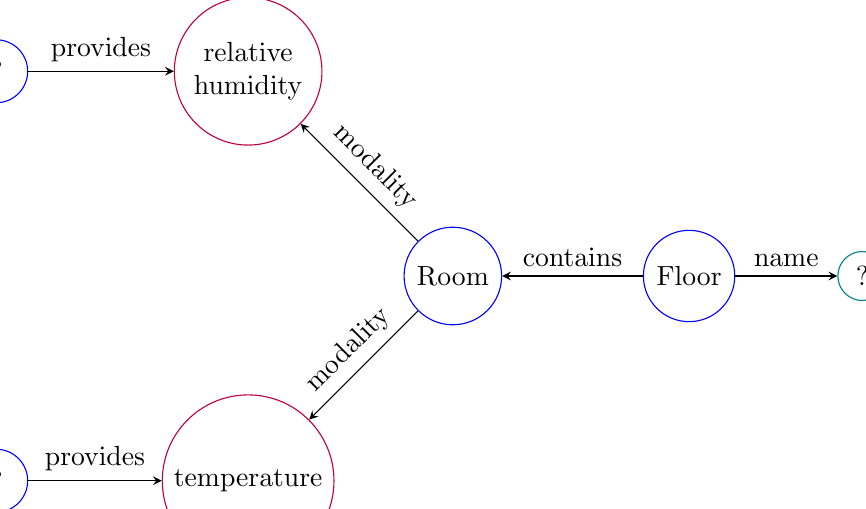
\begin{tikzpicture}[remember picture]
      \tikzstyle{dedge} = [->,>=stealth,draw=black]
      \tikzstyle{dbedge} = [<->,>=stealth,draw=black]
      \tikzstyle{node}=[
        overlay,
        circle,
        align=center,
        anchor=center,
      ]
      \tikzstyle{point}=[
        node,
        draw=blue,
        minimum height=\pointsize,
        minimum width=\pointsize,
      ]
      \tikzstyle{room}=[
        node,
        draw=blue,
        minimum height=\pointsize,
        minimum width=\pointsize,
      ]
      \tikzstyle{modality}=[
        node,
        draw=purple,
      ]
      \tikzstyle{unit}=[
        node,
        draw=teal,
        anchor=center,
      ]
      \tikzstyle{data}=[
        node,
        draw=teal,
        anchor=center,
      ]
      \tikzstyle{field}=[
        data,
        rectangle,
        anchor=center,
      ]
      
      \node[room] (room) at (0,0) {Room};
      \node[room] (floor) at ([xshift=30mm] room.center) {Floor};
      \node[data] (floorname) at ([xshift=22mm] floor.center) {?};
      \draw[dedge] (floor) -- (room) node[midway,sloped,above] {contains};
      \draw[dedge] (floor) -- (floorname) node[midway,sloped,above] {name};
      
      \node[modality] (tmodality) at ([xshift=-26mm, yshift=-26mm] room.center) {temperature};
      \node[modality] (hmodality) at ([xshift=-26mm, yshift= 26mm] room.center) {relative\\humidity};
      \node[room] (tsensor) at ([xshift=-32mm] tmodality.center) {?};
      \node[room] (hsensor) at ([xshift=-32mm] hmodality.center) {?};
      \draw[dedge] (room) -- (tmodality) node[midway,sloped,above] {modality};
      \draw[dedge] (room) -- (hmodality) node[midway,sloped,above] {modality};
      \draw[dedge] (tsensor) -- (tmodality) node[midway,sloped,above] {provides};
      \draw[dedge] (hsensor) -- (hmodality) node[midway,sloped,above] {provides};
    \end{tikzpicture}
  \end{center}
  \vspace{8mm}
  \caption[Example of the pattern of an abstract model query]{Example of the pattern of an abstract model query. It matches combinations of temperature and relative humidity sensors that are associated with a specific room, along with the floor name associated with the floor of that room.}
  \label{fig:topics:info:query:pattern}
\end{figure}

Note that this pattern can be reused on a different model (perhaps covering a different build) and is in no way restricted to a single floor with two rooms.

\subsection{Match Sites}

% main query
As the pattern may match multiple areas of the model and each match captures certain information we need a term to refer to the area of the match. This is called the \textsl{match\idx{Match site} site}. Evaluating a query against a model will result in a list of match sites. Running the previous query against the model of figure \ref{fig:topics:info:model} will result in the match sites from figures \ref{fig:topics:info:match:absI} and \ref{fig:topics:info:match:absII}. Notice how both the query captures the same floor name at both match sites, but different instances of providers of temperature and relative humidity.

% fig: scale vbox of [match site 1, match site 2, all unit matches, all data matches]
\begin{figure}[tbp]
  \centering
  \begin{subfigure}[b]{0.48\textwidth}
    \rotatebox{90}{
      \scalebox{0.5}{
        \begin{tikzpicture}[remember picture]
          \genRoomI{-\centerspacing}{0}{highlight:room,highlight:temp,highlight:hum}
          \genRoomII{\centerspacing}{0}{}
          \genFloor{highlight:floor,highlight:name,highlight:room1}
        \end{tikzpicture}
      }
    }
    \caption{1st match site of absolute humidity query.}
    \label{fig:topics:info:match:absI}
  \end{subfigure}
  \hfill
  \begin{subfigure}[b]{0.48\textwidth}
    \rotatebox{90}{
      \scalebox{0.5}{
        \begin{tikzpicture}[remember picture]
          \genRoomI{-\centerspacing}{0}{}
          \genRoomII{\centerspacing}{0}{highlight:room,highlight:temp,highlight:hump}
          \genFloor{highlight:floor,highlight:name,highlight:room2}
        \end{tikzpicture}
      }
    }
    \caption{2nd match site of absolute humidity query.}
    \label{fig:topics:info:match:absII}
  \end{subfigure}
  \\
  \begin{subfigure}[b]{0.48\textwidth}
    \rotatebox{90}{
      \scalebox{0.5}{
        \begin{tikzpicture}[remember picture]
          \genRoomI{-\centerspacing}{0}{highlight:point,highlight:data}
          \genRoomII{\centerspacing}{0}{highlight:point,highlight:data}
          \genFloor{}
        \end{tikzpicture}
      }
    }
    \caption{Match sites of data query.}
    \label{fig:topics:info:match:data}
  \end{subfigure}
  \hfill
  \begin{subfigure}[b]{0.48\textwidth}
    \rotatebox{90}{
      \scalebox{0.5}{
        \begin{tikzpicture}[remember picture]
          \genRoomI{-\centerspacing}{0}{highlight:point,highlight:unit}
          \genRoomII{\centerspacing}{0}{highlight:point,highlight:unit}
          \genFloor{}
        \end{tikzpicture}
      }
    }
    \caption{Match sites of unit query.}
    \label{fig:topics:info:match:unit}
  \end{subfigure}
  
  \caption[Example of match sites in an abstract information model]{Example of match sites in an abstract information model.}
  \label{fig:topics:info:match}
\end{figure}

% data
These providers are really only anchor points. We don't actually capture the IDs that we are looking after. This is a matter of choice though. While the query could easily be extended to match all the needed information, in this example it is excluded for brevity. Instead, imagine a separate query that captures the relationship between providers and IDs. It would match the sites highlighted in figure \ref{fig:topics:info:match:data}, and then it is a small matter of post-processing\idx{Post processing} to combine the results of the two queries.

% units
However, we might also be interested in the unit\idx{Unit} of the reported values. It might be that one temperature sensor is reporting in \si{\degreeCelsius} and another in \si{\kelvin}. For the purpose of our application we need to treat such readings different. Another query can be used to capture this as seen in figure \ref{fig:topics:info:match:unit}. Again, this can trivially be combined with the information captured by the first two queries. And a production query would likely combine all of them into one.

\subsection{Result Sets}

% text

% fig
\begin{figure}[tbp]
  \centering
  \begin{tabular}{lcc}
    \textbf{Field} & \textbf{Match Site 1} & \textbf{Match Site 2} \\
    Floor & 3rd & 3rd \\
    Temperature unit & \si{\degreeCelsius} & \si{\kelvin} \\
    Temperature live data & 17c5ae15 & b0bc97af \\
    Temperature historical data & 12 & 37 \\
    Relative humidity live data & 65d0be73 & 06ef2490 \\
    Relative humidity historical data & 13 & 22 \\
  \end{tabular}
  \caption{Example of result set in an abstract information model.}
  \label{fig:topics:info:resultset}
\end{figure}

\subsection{Model Reuse and Extension}

% note that the same model can be used for other applications, currently you could calculate the per-floor fractional occupancy, but the model could be extended

% list of examples of extensions: polygons for rooms and floors, physical location of sensors, actuators, electrical distribution trees, who rents/occupies the rooms (and their climate preferences)

\subsection{Building Abstractions}

% automatic stacking of virtual sensors: suite of virtual sensors, querying for relative humidity and matching model+stack of virtual sensors

% automatic unit conversion: query can easily match the unit and extract it, an abstraction could do this automatically and convert to a unit of your choice, this is surprisingly easy

\subsection{Ontologies}
\subsubsection{RDF}
\subsubsection{OWL}
\subsubsection{Select Ontologies}

% brick
\idx{Brick}\url{https://brickschema.org}

% web of things

% schema.org

% QUDT
The QUDT\idx{QUDT}\footnote{\url{https://www.qudt.org}} ontology models units. While it is the de-facto ontology for this, it is not particularly convenient for automatic conversion.

\subsection{Property Graphs}
\subsubsection{Neo4J}

\idx{Neo4j}\url{https://neo4j.com}

\subsection{Query Languages}
\subsubsection{Cypher}
\subsubsection{OpenCypher}

\idx{OpenCypher}\url{https://opencypher.org}

\subsubsection{Gremlin}
\subsubsection{SparQL}


